\newpage
\section{The optimal setup}\label{sec:4:optimal-setup}
With the general framework in hand, the next logical question to ask is, whether the stability against placement-variations can be improved.
The rule of thumb for these optimizations is the following:
Increase the gravitational interaction by either having heavier and larger particles or by reducing the separation distance $L$ without substantial sacrifices of experimental realization.
As an example, the stability increases intuitively by increasing the separation distance $L$. However, this does also increase the time $t_\mathrm{max} \propto L^3$ until the maximum amount of entanglement can be measured which would increase the total time $\sim N t_\mathrm{max}$ of the experiment with $N$ individual measurements.
It is not immediately obvious, how the stability and the maximum possible variations $\Delta \theta_\mathrm{crit}$ and $\Delta L_\mathrm{crit}$ behave for the change in parameters.
In the following section, precisely the dependence of this stability is discussed for altering the orientation $\alpha, \beta$, the particle-shield separation $L$, the mass $M_A = M_B \equiv M$ and the superposition size $\Delta x_A = \Delta x_B \equiv \Delta x$ for two identical particles.


\subsection{Orientation}
One of the arguably easiest parameters to change in the experimental setup is the orientation of the cat-state superpositions, which is quantified by $\alpha, \beta \in [0, \pi)$ in \cref{fig:4:complete-setup}.
As already seen in \cref{fig:2:entanglement-dynamics}, maximal entanglement in the parallel orientation is reached after twice the time compared to the orthogonal orientation.
In general, it is advantageous to aim for the highest entanglement rate and thus the smallest $t_\mathrm{max}(\alpha, \beta)$, as this requires a shorter coherence time and thus reduces the total time of the experiment.
The previous results from \cref{cha:first-look} can be further generalized for an arbitrary orientation $\alpha, \beta$. The logarithmic negativity is given by (derived in \cref{apx:entanglement-orientation})
\begin{equation}
  E_N = \log_2\left(1+\abs{\sin\phi}\right)
\end{equation}
where $\phi$ is now dependent on the orientation and is defined as (for $\Delta x \ll L$)
\begin{equation}\label{eq:4:phi-orientation}
  \phi = \frac{G M_A M_B \Delta x_A \Delta x_B}{8\hbar L^3} t \left(\sin\alpha\sin\beta-\frac{1}{2}\cos\alpha\cos\beta\right) .
\end{equation}
The maximum entanglement $E_N=1$ is reached for $\phi = \pm \pi/2$ and thus after a time
\begin{equation}\label{eq:4:t-max}
  t_\mathrm{max}(\alpha,\beta) = \frac{4\pi \hbar L^3}{G M_A M_B \Delta x_A \Delta x_B}\abs{\sin\alpha\sin\beta - \frac{1}{2}\cos\alpha\cos\beta}^{-1}.
\end{equation}
For the specific symmetric cases $\alpha=\pm \beta$ and $\beta = 0$, the resulting entanglement times are shown in \cref{fig:4:t-max-orientation}.
\begin{figure}[!htbp]
  \centering
  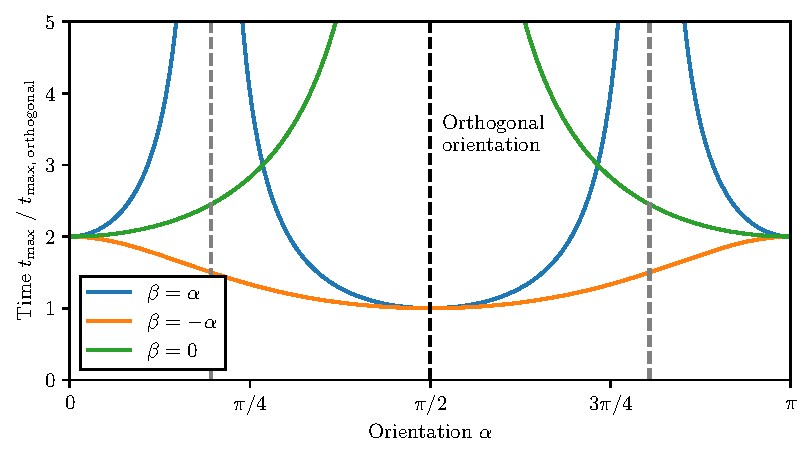
\includegraphics[width=\textwidth]{./../figures/ideal-entanglement/t-max-orientation.pdf}
  \caption{Time $t_\mathrm{max}(\alpha, \beta)$ for different orientations in the special symmetric cases of $\alpha = \pm \beta$ and $\beta = 0$. After this time, a maximally entangled state $E_N = 1$ is reached. The singularity $t_\mathrm{max} \rightarrow \infty$ for $\beta = 0$ and $\alpha = \pi/2$ is expected, as all separations between the cat states $\ket{\psi_A^{(1)}}\leftrightarrow\ket{\psi_B^{(1),(2)}}$ and $\ket{\psi_A^{(2)}}\leftrightarrow\ket{\psi_B^{(1),(2)}}$ is equal. The two other singularities for $\alpha = \beta = 2 \arctan(\sqrt{3} \pm \sqrt{2})$ are explainable by the fact that all separations lie in the \q{harmonic mean}, as seen in \cref{fig:4:harmonic-mean}.}
  \label{fig:4:t-max-orientation}
\end{figure}
The global minima of $t_\mathrm{max}(\alpha,\beta)$ is attained in the orthogonal orientation. This is not surprising considering that this orientation maximizes the \textit{differences in separation distances} between all superposition cat-states.
Much more interesting and unanticipated are the singularities in \cref{fig:4:t-max-orientation} which appear for 
\begin{equation}
  \sin\alpha\sin\beta=\frac{1}{2}\cos\alpha\cos\beta .
\end{equation}
For $\beta=0$ the singularity at $\alpha=\pi/2$ is not surprising. In this configuration, the distances $\ket{\psi^{(1)}_A}\leftrightarrow\ket{\psi^{(1),(2)}_B}$ and $\ket{\psi^{(2)}_A}\leftrightarrow\ket{\psi^{(1),(2)}_B}$ are identical and thus these states accumulate the same phases, resulting in a factorable global phase.
In the case of $\alpha=\beta$, the two singularities are precisely given in the orientation
\begin{equation}
  \alpha=\beta=2 \arctan(\sqrt{3}\pm\sqrt{2})\approx 90\deg \pm 54.74\deg .
\end{equation}
There exists a non-obvious geometric interpretation why no entanglement is generated exactly in this configuration, as all 4 separation distances between the states form the \q{harmonic mean} visualized in \cref{fig:4:harmonic-mean}.
\begin{figure}[!htbp]
  \centering
  \def\svgwidth{\textwidth}
  \input{./../figures/harmonic-mean.pdf_tex}
  \caption{\textbf{left:} The system in the orientation $\alpha=\beta=2\arctan(\sqrt{3}-\sqrt{2})$. For $\Delta x \ll L$, all separation distances exactly form the \textit{harmonic mean}. Here, the phases due to the mutual gravitational interaction precisely cancel out resulting in no entanglement. \textbf{right:} Geometric visualization of the harmonic mean.}
  \label{fig:4:harmonic-mean}
  % COLORFUL:: $\textcolor[HTML]{aa0000}{\blacksquare} = \displaystyle\frac{2}{\frac{1}{\textcolor[HTML]{0044aa}{\blacksquare}}+\frac{1}{\textcolor[HTML]{447821}{\blacksquare}}}$
\end{figure}
In the limit $\Delta x \ll L$, all dynamic phases for the different cat-states can be factored in a global phase and thus resulting in a loss of entanglement. 
To avoid all these singularities, it is advisable to always choose $\alpha=-\beta$, where all orientations result in roughly similar entanglement times $t_\mathrm{max}$, at most only differing by a factor of $2$.

It should come by no surprise that the different orientations exhibit different stabilities. Naturally, one would expect the parallel configuration to be much more sensitive to angular variations than the orthogonal one.
In contrast, the parallel configuration should be much more stable against variations $L$, as no phase difference is induced between the two superposition states $\ket{\psi^{(1)}_{A(B)}}$ and $\ket{\psi^{(2)}_{A(B)}}$ of the particles $A$ and $B$.

The effect of different orientations on the stability against angular variations and the behavior of the critical angular variation $\Delta \theta_\mathrm{crit}$ is shown in \cref{fig:4:theta-crit-orientation}.
\begin{figure}[!htbp]
  \centering
  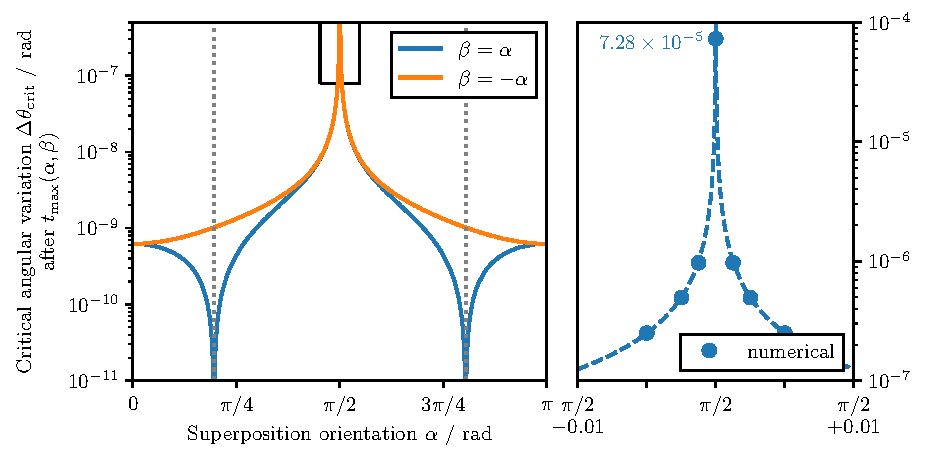
\includegraphics[width=\textwidth]{./../figures/theta-variance/theta-crit-orientation-complete.pdf}
  \caption{Critical angular variation $\Delta \theta_\mathrm{crit}$ for different orientations after the time $t_\mathrm{max}(\alpha, \beta)$. The \emph{orthogonal orientation} magnified on the right is very stable against angular variations and only numerical methods show a finite stability value. The singularities in the left figure for $\alpha = \beta$ arise from the fact, that these orientations need infinite time to entangle as already seen in \cref{fig:4:t-max-orientation}.}
  \label{fig:4:theta-crit-orientation}
\end{figure}
As expected, the orthogonal configuration is the most stable against these kind of variations. This is, because the dephasing ultimately depends on the distance between the cat-state and the shield $L \pm \Delta x/2 \cos\theta \approx L \pm \Delta x/2 (1 - \theta^2/2)$, which is a only second order effect of the angular variations $\theta$.
This explains the apparent \q{infinitely} good stability in the figure, as the analytical solution only uses first order approximations in $\theta$.
Exact numerical results however cap the stability at $\Delta \theta_\mathrm{crit,\,orthogonal} \approx 7.3\times 10^{-5}\si{rad}$.

Respectively, the stability against distance variations $\Delta L_\mathrm{crit}$ for different orientations is shown in \cref{fig:4:L-crit-orientation}.
\begin{figure}[!htbp]
  \centering
  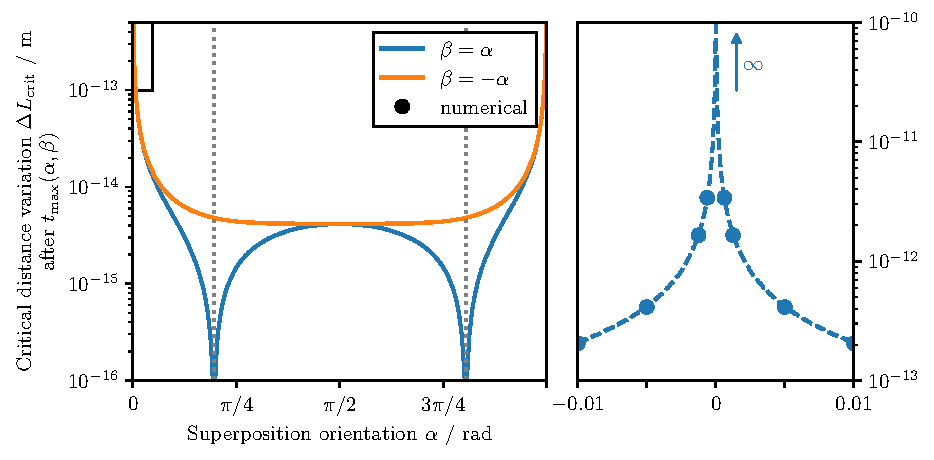
\includegraphics[width=\textwidth]{./../figures/L-variance/L-crit-orientation-complete.pdf}
  \caption{Critical variation in the particle-shield separation $\Delta L_\mathrm{crit}$ for different orientations after a time $t_\mathrm{max}(\alpha,\beta)$. Here, the \emph{parallel orientation} (magnified on the right) is \q{infinitely} stable against placement variations.}
  \label{fig:4:L-crit-orientation}
\end{figure}
Again aligning with expectations, the parallel configuration exhibits an infinite stability.
One could argue, that a for this to hold, the uncertainties in the angular placement have to be zero. As however seen in \cref{fig:4:theta-crit-orientation}, these variations are at most around $\sim 5 \times 10^{-5}\si{rad}$ and thus a realistic upper bound for the minimum required distance variations is given by $\Delta L_\mathrm{crit,parallel} = \Delta L_\mathrm{crit}(\alpha \approx 5\times 10^{-5}\si{rad}) \simeq 4\times 10^{-11}\si{m}$.
It is important to keep in mind, that these bounds can be improved substantially by e.g. increasing the separation distance $L$, the particle size $R$ or the superposition size $\Delta x$.

Considering these results, the parallel orientation seems to be the more stable and therefore favorable option, even if the required coherence times $t_\mathrm{max}$ are twice as long.
Keeping particle-shield separation variations below $0.01\si{pm}$ in the orthogonal orientation - even smaller than size of a single atom - is extremely challenging,  
especially under the additional consideration of the thermal vibrations of the shield, which are in the same order of magnitude as seen later in \cref{cha:the-shield}.
With this framework on hand, it is possible to generate the stability diagram in \cref{fig:4:optimal-orientation}, showing the optimal orientation in which the most entanglement can be measured.
For most combinations of $\Delta L$ and $\Delta \theta$, entanglement is exclusively given in either the parallel or orthogonal orientation.
\begin{figure}[!htbp]
  \centering
  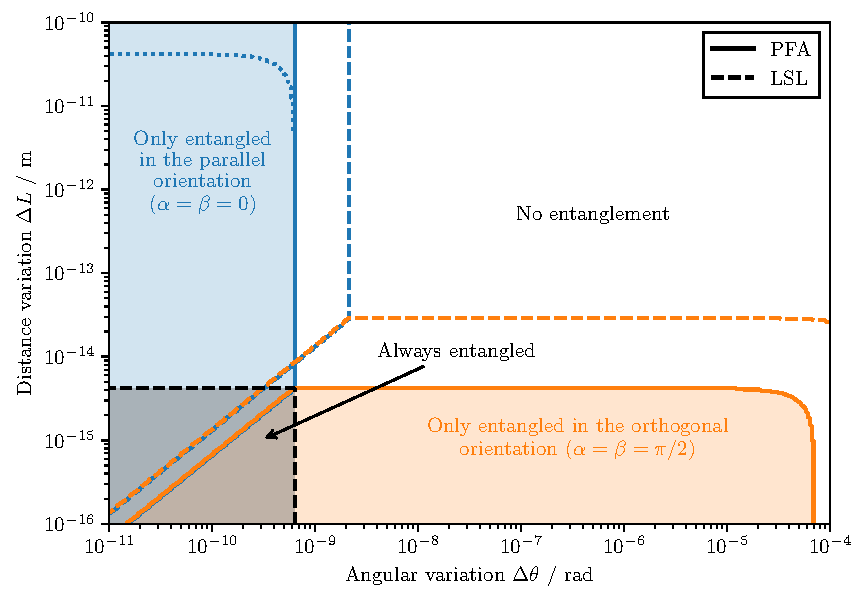
\includegraphics[width=\textwidth]{./../figures/optimize/optimized-orientation-advanced.pdf}
  \caption{Optimal and most stable configuration for the orientation of the cat-states relative to the shield for different variations in the angle $\Delta \theta$ and in the separation distance $\Delta L$. The used parameters for the particle are shown in \cref{tab:paramters} and e.g. larger separations $L$ would improve the stability boundaries significantly. Both models for the Casimir interactions are shown. In regions where entanglement is given regardless of the orientation (bottom left), the the favorable orientation with \q{more} entanglement is colored. The blue dotted line corresponds to the realistic upper bound discussed in the text, where an additional angular variation of $5 \times 10^{-5}\si{rad}$ as a worst-case estimation is assumed.}
  \label{fig:4:optimal-orientation}
\end{figure}


\newpage
\subsection{Separation, mass and superposition size}
It is possible to improve the placement accuracies required in the initial placement of the particles by changing the parameters in \cref{tab:paramters}.
The particle-shield separation $L$ in particular can be adjusted easily over a wide range and one is only limited in the ability of trapping close to the shield (discussed in \cref{sec:4:trapping}) and the size of the experimental setup.
The scaling of the critical angular variation $\Delta \theta_\mathrm{crit}$, above which no entanglement is generated anymore, for different $L$ is shown in \cref{fig:4:theta-crit-L}.
\begin{figure}[!htbp]
  \centering
  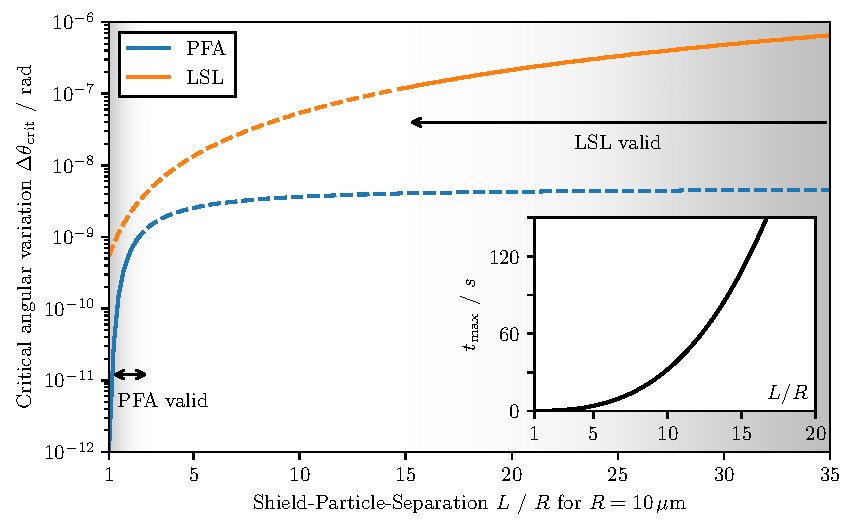
\includegraphics[width=\textwidth]{./../figures/theta-variance/theta-crit-L.pdf}
  \caption{Stability against angular variations for increasing separation distances $L$ in units of $R=10\si{\mu m}$ after a time $t_\mathrm{max}(L)$. The dependence on the radius can be seen in \cref{fig:4:theta-crit-mass}. Two models for the Casimir-interaction are shown: The proximity-force-approximation (PFA) and the large-separation-limit (LSL). The regions outside the models validity are indicated with dashed lines. In the bottom right the time $t_\mathrm{max}(L) \propto L^3$ is shown.}
  \label{fig:4:theta-crit-L}
\end{figure}
A similar figure can be created for the change of $\Delta L_\mathrm{crit}$, but as already discussed previously, the setup in the parallel orientation is very stable against variations in the separation distance, so only angular variations have to be considered.

It is intuitively clear, that a larger separation improves the stability as the relative effect of the angular variations $\sim \Delta x \sin\theta \ll L$ decreases and the Casimir potential tends towards zero.
However, a larger separation also slows down the entanglement generation by $t_\mathrm{max} \propto L^3$.
The combination of both effects leads to the results shown in \cref{fig:4:theta-crit-L}.
Both models for the Casimir interaction for either small separations $L \sim R$ (PFA) or large separations $L \gg R$ (LSL) have been considered and the regions of validity for each model are shaded in gray.
Looking at the dependence of the critical point eq. \eqref{eq:4:critical-point} on the separation, it becomes evident that ($\xi$ is given by eq. \eqref{eq:apx:definition-xi})
\begin{equation}
  \Delta \theta_\mathrm{crit} \sim 1/(\xi t) \sim \frac{(L - R - d/2)^3}{t_\mathrm{max}} \sim \frac{(L - R - d/2)^3}{L^3}
\end{equation}
for small separations and similarly $\Delta \theta_\mathrm{crit} \sim L^2$.
For this approximations, it was additionally used that the Casimir force is much larger than the gravitational interaction for all $L \lesssim 3.2\si{m}$ (in \cref{fig:4:theta-crit-L}, the match is quantified by $R^2 = 0.99$).

Contrary to $L$, the size of the particle $R$ and thus the mass $M$ cannot be changed easily over a wide range of possible values.
Estimations suggest, that masses of around $10^{-11}\si{kg} \approx 5 \times 10^{-4}m_p$ could be possible to use for the detection of gravitationally induced entanglement \cite[Timestamp 51:00]{Aspelmeyer_2024}.
Nevertheless, the effect of a larger particle on angular variations is analyzed and shown in \cref{fig:4:theta-crit-mass}.
\begin{figure}[!htbp]
  \centering
  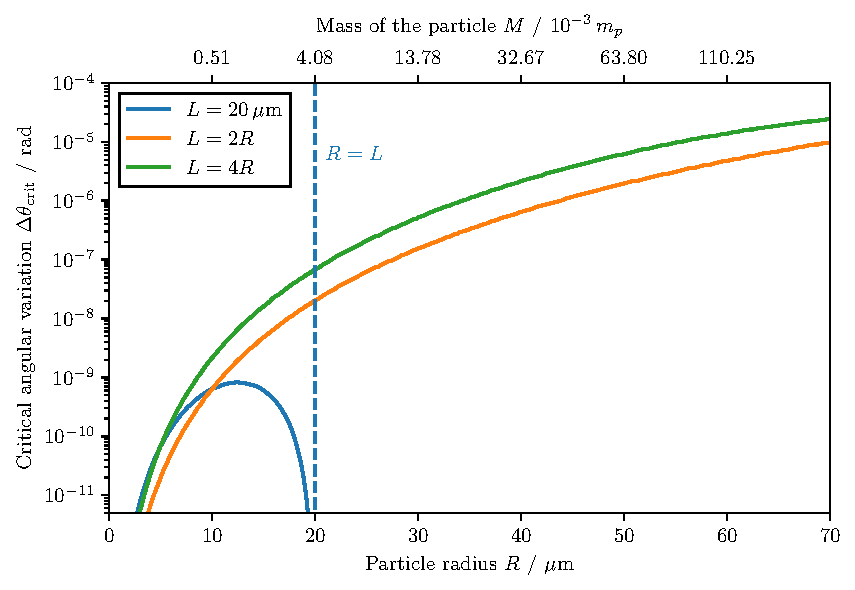
\includegraphics[width=\textwidth]{./../figures/theta-variance/theta-crit-mass.pdf}
  \caption{Critical angular variation $\Delta \theta_\mathrm{crit}$ for different sized particles after a time $t_\mathrm{max}(M)$. The mass of the corresponding particle in units of the Planck mass $m_p = \sqrt{\hbar c / G} \approx 2.176\times 10^{-8}\si{kg}$ is given on the top axis. For particles as large as the separation $R = L$, the surface-to-surface separation is almost zero, resulting in large Casimir forces and thus no entanglement.}
  \label{fig:4:theta-crit-mass}
\end{figure}
The particles are most likely made out of silica ($\mathrm{SiO_2}$) with density $\rho_\mathrm{Silica} = 2648\si{kg/m^3}$, as this material has been widely used in experiments on levitated nanoparticles \cite{Grass_2016,Slezak_2018}.
Denser materials like lead or osmium \cite{Krisnanda_2020} in magnetic traps could potentially be considered as the required particle radius and the number of atoms in a single particle are reduced.
The entanglement generation fastens substantially for larger particles as $t_\mathrm{max}$ scales with $M^{-2}$ and thus effectively with $R^{-6}$ (of course only if $L$ is independent of $R$).
The dependence of $\Delta \theta_\mathrm{crit}$ on $R$ can be determined in first order to
\begin{equation}
  \Delta \theta_\mathrm{crit} \sim \frac{(L - R - d/2)^3}{R t_\mathrm{max}} \sim \frac{(L - R - d/2)^3 R^6}{R L^3 }
\end{equation}
for small separations and in the special case where $L \propto R$, a scaling of $\Delta \theta_\mathrm{crit} \sim (R - d/2)^3 R^2$ is expected.
Both cases are shown in \cref{fig:4:theta-crit-mass}.

Similarly to the particles size, the spatial extension of the coherent superposition of the center-of-mass motion $\Delta x$ can most likely not be changed substantially. The delocalizations are, considering the current record in matter-wave experiments of $500\si{nm}$ for $4\times 10^{-23}\si{kg}$ \cite{Fein_2019}. It remains to be seen what superposition sizes are possible to create using levitated particles.  
In \cref{fig:4:theta-crit-superposition-size} the effect of the superposition size on the critical angular variation is shown.
\begin{figure}[!htbp]
  \centering
  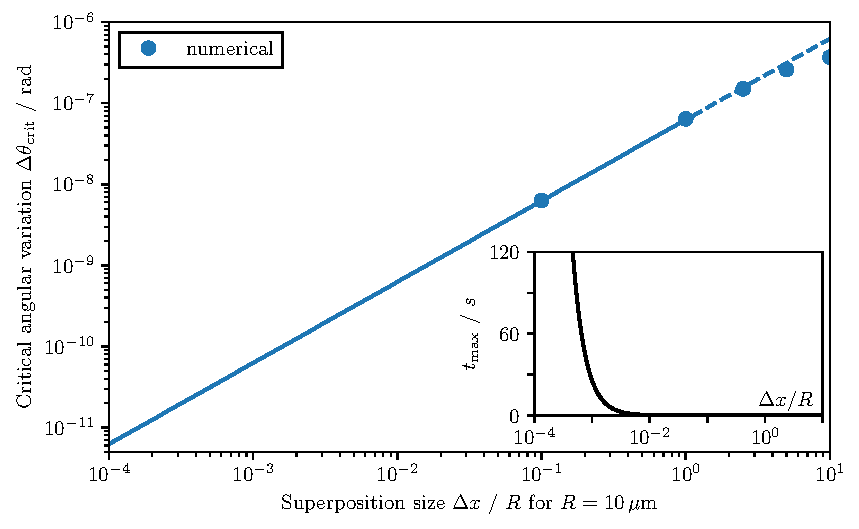
\includegraphics[width=\textwidth]{./../figures/theta-variance/theta-crit-superpos-size.pdf}
  \caption{Effect of the superposition size $\Delta x$ on the critical angular stability $\Delta \theta_\mathrm{crit}$ after a time $t_\mathrm{max}(\Delta x)$. For $\Delta x \gtrsim R$, numerical results are used. In the lower left, the time $t_\mathrm{max} \propto (\Delta x)^{-2}$ is shown, until maximum entanglement is reached. For $\Delta x \ll R$, the resulting relation between $\Delta x$ and $\Delta \theta_\mathrm{crit}$ is linear.}
  \label{fig:4:theta-crit-superposition-size}
\end{figure}
A larger superposition would increase the entanglement generation as the relative phase differences between the states increase, leading to $t_\mathrm{max} \propto 1/(\Delta x)^{2}$. 
Simultaneously, a larger superposition size increases the effect of angular variations, as they depend on $\sim \Delta x \sin(\theta)$.
The effective scaling of the angular variations is therefore linear $\Delta \theta_\mathrm{crit} \sim \Delta x$, as seen in \cref{fig:4:theta-crit-superposition-size} \footnote{Here it is shown in a double-logarithmic plot. The relation between $\Delta x$ and $\Delta \theta_\mathrm{crit}$ is nevertheless linear.}.



